\section{Unbalanced Tree Search}
\label{sec:uts}

The Unbalanced Tree Search benchmark (UTS) measures the rate of traversal of
a tree generated on the fly using a splittable random number
generator \cite{lcpc06}. Each node in the tree is identified by a 160-bit hash.
The UTS specification describes several cryptographic laws for computing the number of children of a node and their hashes.
The intent is to synthesize trees that are deterministic but unbalanced in unpredictable ways. 

A sequential implementation of UTS is straightforward. The code maintains a work list of pending nodes to visit, initialized with the root node of the tree. It repeatedly pops a node from the work list, computes the list of children for this node, and adds them to the work list, while keeping the count of the nodes processed so far. An empty work list signals the termination of the traversal.
In contrast, a parallel and distributed implementation of UTS is a challenge because of imbalance.
We implement distributed work stealing with lifelines \cite{ppopp11}.

\paragraph{Distributed Algorithm.} A fixed collection of workers collaborate on the traversal. The workers are organized in a ring.
Each worker maintains a work list of pending nodes to visit and count of nodes already traversed. Each worker primarily processes its own list, following the sequential algorithm. If the list becomes empty, the worker tries to steal nodes from another random worker. If this fails because the victim's work list is empty as well, the worker sends a request to the next worker in the ring---its lifeline---and stops. If this lifeline now has or later obtains nodes to process, it deals a fraction of these nodes to the requester. One work list is initialized with the root node of the traversal. The traversal is complete when all workers have stopped and there are no deal messages from a lifeline in flight. The sum of the node counts is computed at that point.

\paragraph{State Machine.} Each worker can be in one of three states:
\begin{itemize}
\item work: the worker is processing nodes from its work list;
\item wait: the worker is attempting to steal nodes from a random victim and waiting for the result;
\item idle: the worker has signaled its lifeline and stopped.
\end{itemize}
Figure~\ref{fig:uts-state} shows these states and the possible transitions as a graph. The transitions---the edges---are annotated with the events associated with them. E.g., the ``nodeal/lifelinereq'' transition from the wait state to the idle state denotes that this transition takes places upon receiving the ``nodeal'' message and involves sending the ``lifelinereq'' message.

\begin{figure}
\centering
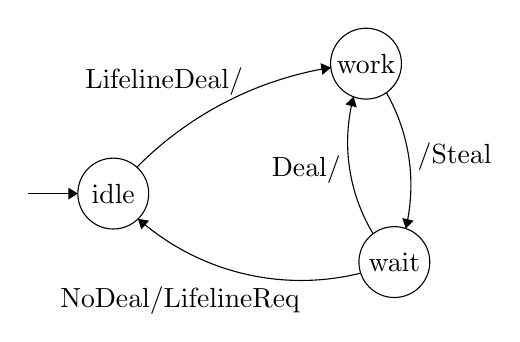
\begin{tikzpicture}[scale=0.15]
\tikzstyle{every node}+=[inner sep=0pt]
\draw [black] (20.9,-23.3) circle (3);
\draw (20.9,-23.3) node {idle};
\draw [black] (42.3,-12.3) circle (3);
\draw (42.3,-12.3) node {work};
\draw [black] (44.7,-29.1) circle (3);
\draw (44.7,-29.1) node {wait};
\draw [black] (22.9,-21.066) arc (135.27934:99.12868:29.75);
\fill [black] (39.32,-12.63) -- (38.45,-12.26) -- (38.61,-13.25);
\draw (25.2,-15.02) node [above] {\lstinline{LifelineDeal}/};
%\draw [black] (43.382,-9.514) arc (186.50322:-101.49678:2.25);
%\fill [black] (45.17,-11.46) -- (46.02,-11.87) -- (45.91,-10.88);
\draw [black] (44.023,-14.75) arc (29.69026:-13.43006:15.827);
\fill [black] (45.67,-26.27) -- (46.34,-25.6) -- (45.37,-25.37);
\draw (46.63,-20.18) node [right] {/\lstinline{Steal}};
\draw [black] (42.903,-26.704) arc (-148.86241:-194.87738:14.991);
\fill [black] (41.25,-15.1) -- (40.56,-15.75) -- (41.52,-16);
\draw (40.2,-21.24) node [left] {\lstinline{Deal}/};
\draw [black] (41.852,-30.034) arc (-75.95772:-131.43403:20.846);
\fill [black] (23,-25.44) -- (23.27,-26.34) -- (23.93,-25.59);
\draw (26.55,-31.11) node [below] {\lstinline{NoDeal}/\lstinline{LifelineReq}};
\draw [black] (13.7,-23.3) -- (17.9,-23.3);
\fill [black] (17.9,-23.3) -- (17.1,-22.8) -- (17.1,-23.8);
\end{tikzpicture}
\caption{State diagram for UTS workers.\label{fig:uts-state}}
\end{figure}

\paragraph{Distributed Termination.} Distributed termination detection is notoriously difficult to implement correctly and efficiently.
For instance in UTS, observing that all workers are idle does not guarantee that the traversal is complete as messages containing nodes to process might still be in flight. Thanks to \lstinline{finish}, an entire class of hard-to-reproduce data races is ruled out by construction in APGAS.
A combination of static and dynamic analyses can bring down the cost of termination detection~\cite{TardieuETAL14X10ApgasAtPetascale}. 

APGAS provides two state-of-the-art \lstinline{finish} implementations for fault-tolerant and non-fault-tolerant instantiations of the library. The core algorithm uses a distributed array of counters akin to the X10 implementation. Each place maintains the count of tasks that completed locally and separate counts for each place where it spawned tasks. These arrays of counters are pushed to the place of the task waiting on the \lstinline{finish}. Termination is signaled when all the sums of the per-place task counts are zero.


TODO

Common implementation of WorkList. Show interface. Explain mutability and
ownership are for performance.

Akka: implementation using vanilla actors (no akka-fsm). Work is split up by
sending \lstinline{Work} messages to oneself. State transitions are implemented
using \lstinline{become}.

Termination is difficult.

UTS: three problems, three solutions.

UTS \apgas: concurrency control implemented as multiple paradigms (synchronized
data access, global invariants, active messages). Concurrency is more
fine-grained.


% Scala performance

%UTSAPGAS 32 places, 1 worker/place, depth 15
%[uts-apgas-32] depth: 15, performance: 4230646601/15.617225935 = 270.8961641848719M nodes/s
%[uts-apgas-32] depth: 15, performance: 4230646601/15.757630678 = 268.4824062355144M nodes/s
%[uts-apgas-32] depth: 15, performance: 4230646601/15.730685914 = 268.9422841527087M nodes/s

%UTSAkka 32 process, 1 actor/process, depth 15
%[actors-32] depth: 15, performance: 4230646601/15.605088175 = 271.1068693464784M nodes/s
%[actors-32] depth: 15, performance: 4230646601/15.478703563 = 273.3204744041263M nodes/s
%[actors-32] depth: 15, performance: 4230646601/15.208430648 = 278.1777225355172M nodes/s

%UTSAkka 1 process, 32 actors, depth 15
%[actors-32] depth: 15, performance: 4230646601/14.622429161 = 289.32584007886373M nodes/s
%[actors-32] depth: 15, performance: 4230646601/14.783925108 = 286.16531605065273M nodes/s
%[actors-32] depth: 15, performance: 4230646601/14.852197401 = 284.8498768751316M nodes/s


%UTSSequential depth 13
%[serial] depth: 13, performance: 264459392/27.782491057 = 9.518922959695061M nodes/s
%[serial] depth: 13, performance: 264459392/27.740853577 = 9.533210334207734M nodes/s
%[serial] depth: 13, performance: 264459392/27.538216937 = 9.603359309900553M nodes/s


% Java performance

%GlobalUTS 32 places, 1 worker/place, depth 15 (hacked non resilient)
%Depth: 15, Places: 32, Performance: 4230646601/15.191 = 278.48M nodes/s using 0 transactions
%Depth: 15, Places: 32, Performance: 4230646601/15.267 = 277.09M nodes/s using 0 transactions
%Depth: 15, Places: 32, Performance: 4230646601/15.138 = 279.46M nodes/s using 0 transactions

%MultiUTS 1 place, 32 workers, depth 15 (hacked non resilient)
%Depth: 15, Locations: 32, Performance: 4230646601/14.601 = 289.73M nodes/s using 0 transactions
%Depth: 15, Locations: 32, Performance: 4230646601/14.791 = 286.02M nodes/s using 0 transactions
%Depth: 15, Locations: 32, Performance: 4230646601/14.557 = 290.61M nodes/s using 0 transactions

%GlobalUTS 32 places, 1 worker/place, depth 15 (resilient map)
%Depth: 15, Places: 32, Performance: 4230646601/15.883 = 266.35M nodes/s using 1119 transactions

